\section{شرح پروژه}
در این پروژه ما یک سامانه‌ی 
\lr{iot}
رصد وضعیت هوا طراحی کردیم که وضعیت 3 نوع گاز سمی در هوا را اندازه‌‌گیری می‌کند و با توجه به مقادیر این گاز‌ها اخطار‌های لازم را به کاربران می‌دهد. این سامانه اطلاعات وضعیت هوا را از تعدادی دستگاه که هر یک سه سنسور مخصوص به گاز ‌دارند می‌گیرد و میانگین وضعیت آن‌ها را نشان می‌دهد و بر اساس وضعیت گاز با بیشترین غلظت وضعیت آلودگی کلی را نشان می‌دهد. این سامانه به صورت یک اپلیکیشن گوشی پیاده‌سازی شده است که با یک لوکیشن خاص کار می‌کند و همچنین یک وب‌سرور که اطلاعات میانگین چند دستگاه را نمایش می‌دهد. شمای کلی طراحی را در شکل زیر مشاهده می‌کنید. 
\begin{figure}[h!]
	\centering		
	\includegraphics[width=\linewidth]{figs/iot.png}
	\caption{شمای کلی سیستم}
\end{figure}


\subsection{تغییرات نسبت به پروپوزال اولیه}
در پروپوزال پروژه ما سیستم را به صورت یک دستگاه در نظر گرفتیم اما در ارائه‌ی اولیه تصمیم بر آن شد که قابلیت داشتن دستگاه در چند لوکیشن مختلف را نیز پیاده‌سازی کنیم. بنابراین ما یک وب سرور طراحی کردیم که بتواند مقادیر گاز‌ها را از چند برد مختلف در لوکیشن‌های مختلف بگیرد و میانگین آن‌ها را گزارش دهد که مشابه کاری است که دستگاه‌های رصد هوای مزاکر مناطق مختلف شهر انجام می‌دهند. همچنین اپلیکیشن گوشی نیز طراحی کردیم که مطابق آنچه در پروپوزال گفته شده بود از یک دستگاه آمار را می‌گیرد و مشابه یک سامانه رصد هوای خانگی برای ساختمان‌های هوشمند عمل می‌کند.  

\section{طراحی و پیاده سازی}
- کلا iot builder و این داستانا رو یه ذره بگیم و نوع پروژه توی پرتئوس و اینا

در این پروژه ما با استفاده از 
\href{https://labcenter.s3.amazonaws.com/downloads/iotHelp.pdf}{iot-builder}
یک 
\subsection{شماتیک مدار}
شماتیک مدار را در شکل زیر مشاهده می‌کنید. در این مدار یک برد 
\lr{Arduino Yun}
که برای کاربرد‌های 
\lr{iot}
مناسب است و سه سنسور
\lr{LM35DZ}
تعبیه شده است که سنسور‌های دما هستند اما ما از آن‌ها به عنوان سنسور تشخیص گاز استفاده می‌کنیم. در پروپوزال ما سنسور‌های واقعی اندازه‌گیری گاز 
\lr{MQ-7}
و 
\lr{MQ-2}
و
\lr{MQ-135}
را استفاده کرده بودیم اما چون این سنسور‌ها در 
\lr{Proteus}
نبودند ما از سنسور‌های جایگزین اندازه‌گیری دما استفاده کردیم.
\begin{figure}[h!]
	\centering		
	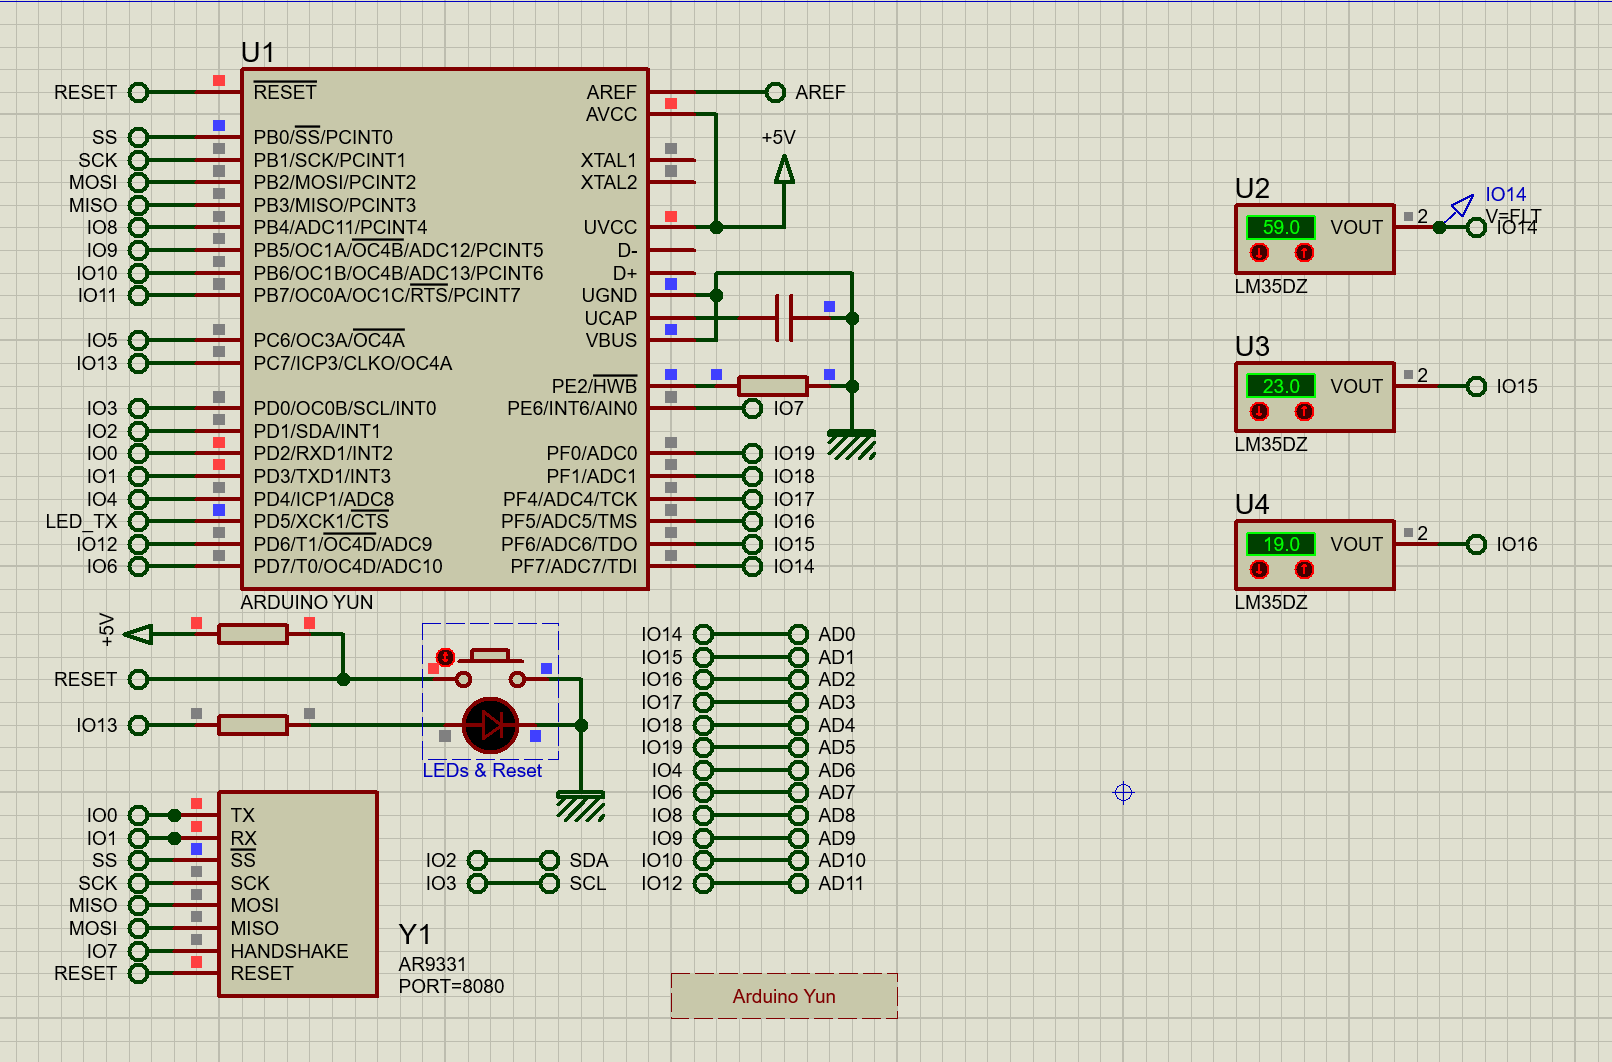
\includegraphics[width=\linewidth]{figs/circuit.png}
	\caption{شماتیک مدار}
\end{figure}

\subsection{توضیح کلی کد}
اینجا کلا توضیج میدیم که کد چه جوریه و سیستم چه جوریه و اینا

\subsection{اپلیکیشن گوشی}
برای طراحی اپلیکیشن گوشی ما از قابلیت‌های 
\lr{Visual Designer}
استفاده کردیم و کنترلر‌های 
\lr{iot}
زیر را 

- عکس از پنل گوشی

- توضیج این که چطوری از طریق وای فای با اضافه کردن ip دستگاه از روی گوشی ریزالتو می بینیم و اینا

\subsection{وب‌سرور و میانگین‌گیری از نتایج چند دستگاه}
- اینجا راجع به  
elastic search
 اینا توضیح میدیم و ساختن ایندکسو پوش کردن ریزالتا و ...

\section{فایل‌ها و شیوه ‌ی اجرای برنامه}
- اینجا یه توضیحی میدیم که کلا فایلا چین و کی کجاست و ران گرفتن چه جوریه. من یه سری فایل برای الستیک هم گذاشتم برای ساخت ایندکس و اینا. 

\section{سیمولیشن و نتایج}
- یه تعدادی عکس از اجرای برنامه از روی گوشی با یه لوکیشن و از روی وب سرور با مثلا دو تا لوکیشن


\section{چالش‌ها}